% Created by tikzDevice version 0.10.1 on 2016-09-09 18:45:25
% !TEX encoding = UTF-8 Unicode
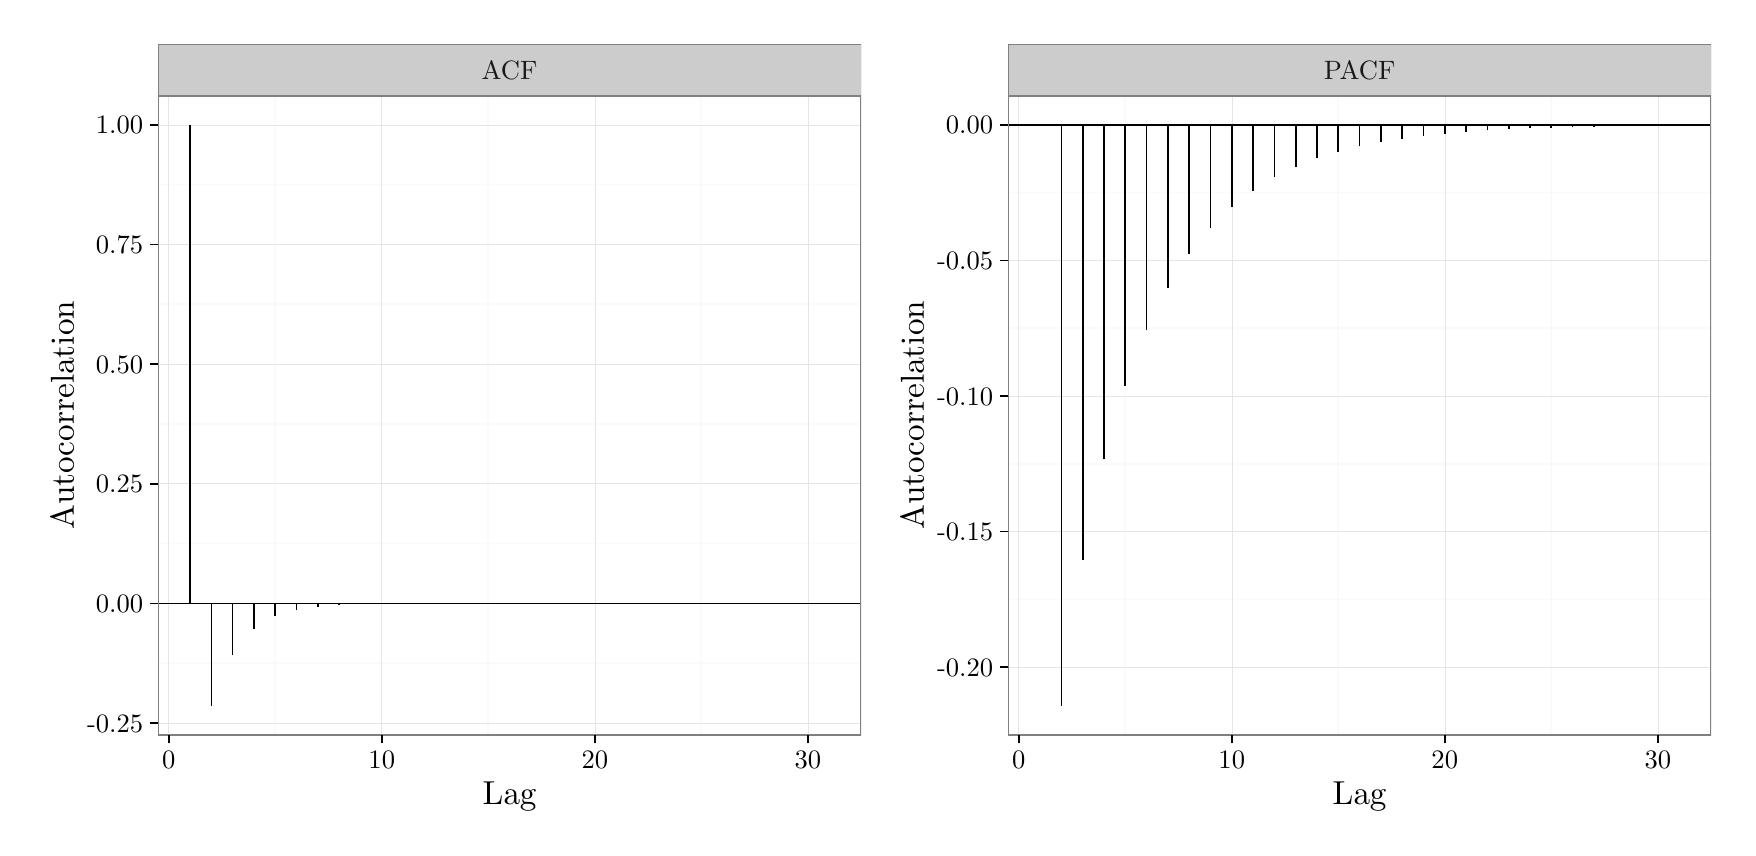
\begin{tikzpicture}[x=1pt,y=1pt]
\definecolor{fillColor}{RGB}{255,255,255}
\path[use as bounding box,fill=fillColor,fill opacity=0.00] (0,0) rectangle (614.29,289.08);
\begin{scope}
\path[clip] (  0.00,  0.00) rectangle (307.15,289.08);
\definecolor{drawColor}{RGB}{255,255,255}
\definecolor{fillColor}{RGB}{255,255,255}

\path[draw=drawColor,line width= 0.6pt,line join=round,line cap=round,fill=fillColor] (  0.00,  0.00) rectangle (307.15,289.08);
\end{scope}
\begin{scope}
\path[clip] ( 47.13, 33.48) rectangle (301.15,264.47);
\definecolor{fillColor}{RGB}{255,255,255}

\path[fill=fillColor] ( 47.13, 33.48) rectangle (301.15,264.47);
\definecolor{drawColor}{gray}{0.98}

\path[draw=drawColor,line width= 0.6pt,line join=round] ( 47.13, 59.42) --
	(301.15, 59.42);

\path[draw=drawColor,line width= 0.6pt,line join=round] ( 47.13,102.65) --
	(301.15,102.65);

\path[draw=drawColor,line width= 0.6pt,line join=round] ( 47.13,145.88) --
	(301.15,145.88);

\path[draw=drawColor,line width= 0.6pt,line join=round] ( 47.13,189.12) --
	(301.15,189.12);

\path[draw=drawColor,line width= 0.6pt,line join=round] ( 47.13,232.35) --
	(301.15,232.35);

\path[draw=drawColor,line width= 0.6pt,line join=round] ( 89.46, 33.48) --
	( 89.46,264.47);

\path[draw=drawColor,line width= 0.6pt,line join=round] (166.44, 33.48) --
	(166.44,264.47);

\path[draw=drawColor,line width= 0.6pt,line join=round] (243.42, 33.48) --
	(243.42,264.47);
\definecolor{drawColor}{gray}{0.90}

\path[draw=drawColor,line width= 0.2pt,line join=round] ( 47.13, 37.80) --
	(301.15, 37.80);

\path[draw=drawColor,line width= 0.2pt,line join=round] ( 47.13, 81.03) --
	(301.15, 81.03);

\path[draw=drawColor,line width= 0.2pt,line join=round] ( 47.13,124.27) --
	(301.15,124.27);

\path[draw=drawColor,line width= 0.2pt,line join=round] ( 47.13,167.50) --
	(301.15,167.50);

\path[draw=drawColor,line width= 0.2pt,line join=round] ( 47.13,210.73) --
	(301.15,210.73);

\path[draw=drawColor,line width= 0.2pt,line join=round] ( 47.13,253.97) --
	(301.15,253.97);

\path[draw=drawColor,line width= 0.2pt,line join=round] ( 50.98, 33.48) --
	( 50.98,264.47);

\path[draw=drawColor,line width= 0.2pt,line join=round] (127.95, 33.48) --
	(127.95,264.47);

\path[draw=drawColor,line width= 0.2pt,line join=round] (204.93, 33.48) --
	(204.93,264.47);

\path[draw=drawColor,line width= 0.2pt,line join=round] (281.90, 33.48) --
	(281.90,264.47);
\definecolor{drawColor}{RGB}{0,0,0}

\path[draw=drawColor,line width= 0.6pt,line join=round] ( 47.13, 81.03) -- (301.15, 81.03);

\path[draw=drawColor,line width= 0.6pt,line join=round] ( 58.67,253.97) -- ( 58.67, 81.03);

\path[draw=drawColor,line width= 0.6pt,line join=round] ( 66.37, 43.98) -- ( 66.37, 81.03);

\path[draw=drawColor,line width= 0.6pt,line join=round] ( 74.07, 62.50) -- ( 74.07, 81.03);

\path[draw=drawColor,line width= 0.6pt,line join=round] ( 81.77, 71.77) -- ( 81.77, 81.03);

\path[draw=drawColor,line width= 0.6pt,line join=round] ( 89.46, 76.40) -- ( 89.46, 81.03);

\path[draw=drawColor,line width= 0.6pt,line join=round] ( 97.16, 78.72) -- ( 97.16, 81.03);

\path[draw=drawColor,line width= 0.6pt,line join=round] (104.86, 79.88) -- (104.86, 81.03);

\path[draw=drawColor,line width= 0.6pt,line join=round] (112.56, 80.45) -- (112.56, 81.03);

\path[draw=drawColor,line width= 0.6pt,line join=round] (120.25, 80.74) -- (120.25, 81.03);

\path[draw=drawColor,line width= 0.6pt,line join=round] (127.95, 80.89) -- (127.95, 81.03);

\path[draw=drawColor,line width= 0.6pt,line join=round] (135.65, 80.96) -- (135.65, 81.03);

\path[draw=drawColor,line width= 0.6pt,line join=round] (143.35, 81.00) -- (143.35, 81.03);

\path[draw=drawColor,line width= 0.6pt,line join=round] (151.04, 81.02) -- (151.04, 81.03);

\path[draw=drawColor,line width= 0.6pt,line join=round] (158.74, 81.02) -- (158.74, 81.03);

\path[draw=drawColor,line width= 0.6pt,line join=round] (166.44, 81.03) -- (166.44, 81.03);

\path[draw=drawColor,line width= 0.6pt,line join=round] (174.14, 81.03) -- (174.14, 81.03);

\path[draw=drawColor,line width= 0.6pt,line join=round] (181.83, 81.03) -- (181.83, 81.03);

\path[draw=drawColor,line width= 0.6pt,line join=round] (189.53, 81.03) -- (189.53, 81.03);

\path[draw=drawColor,line width= 0.6pt,line join=round] (197.23, 81.03) -- (197.23, 81.03);

\path[draw=drawColor,line width= 0.6pt,line join=round] (204.93, 81.03) -- (204.93, 81.03);

\path[draw=drawColor,line width= 0.6pt,line join=round] (212.63, 81.03) -- (212.63, 81.03);

\path[draw=drawColor,line width= 0.6pt,line join=round] (220.32, 81.03) -- (220.32, 81.03);

\path[draw=drawColor,line width= 0.6pt,line join=round] (228.02, 81.03) -- (228.02, 81.03);

\path[draw=drawColor,line width= 0.6pt,line join=round] (235.72, 81.03) -- (235.72, 81.03);

\path[draw=drawColor,line width= 0.6pt,line join=round] (243.42, 81.03) -- (243.42, 81.03);

\path[draw=drawColor,line width= 0.6pt,line join=round] (251.11, 81.03) -- (251.11, 81.03);

\path[draw=drawColor,line width= 0.6pt,line join=round] (258.81, 81.03) -- (258.81, 81.03);

\path[draw=drawColor,line width= 0.6pt,line join=round] (266.51, 81.03) -- (266.51, 81.03);

\path[draw=drawColor,line width= 0.6pt,line join=round] (274.21, 81.03) -- (274.21, 81.03);

\path[draw=drawColor,line width= 0.6pt,line join=round] (281.90, 81.03) -- (281.90, 81.03);

\path[draw=drawColor,line width= 0.6pt,line join=round] (289.60, 81.03) -- (289.60, 81.03);
\definecolor{drawColor}{gray}{0.50}

\path[draw=drawColor,line width= 0.6pt,line join=round,line cap=round] ( 47.13, 33.48) rectangle (301.15,264.47);
\end{scope}
\begin{scope}
\path[clip] ( 47.13,264.47) rectangle (301.15,283.08);
\definecolor{drawColor}{gray}{0.50}
\definecolor{fillColor}{gray}{0.80}

\path[draw=drawColor,line width= 0.2pt,line join=round,line cap=round,fill=fillColor] ( 47.13,264.47) rectangle (301.15,283.08);
\definecolor{drawColor}{gray}{0.10}

\node[text=drawColor,anchor=base,inner sep=0pt, outer sep=0pt, scale=  0.96] at (174.14,270.47) {ACF};
\end{scope}
\begin{scope}
\path[clip] (  0.00,  0.00) rectangle (614.29,289.08);
\definecolor{drawColor}{RGB}{0,0,0}

\node[text=drawColor,anchor=base east,inner sep=0pt, outer sep=0pt, scale=  0.96] at ( 41.73, 34.49) {-0.25};

\node[text=drawColor,anchor=base east,inner sep=0pt, outer sep=0pt, scale=  0.96] at ( 41.73, 77.73) {0.00};

\node[text=drawColor,anchor=base east,inner sep=0pt, outer sep=0pt, scale=  0.96] at ( 41.73,120.96) {0.25};

\node[text=drawColor,anchor=base east,inner sep=0pt, outer sep=0pt, scale=  0.96] at ( 41.73,164.20) {0.50};

\node[text=drawColor,anchor=base east,inner sep=0pt, outer sep=0pt, scale=  0.96] at ( 41.73,207.43) {0.75};

\node[text=drawColor,anchor=base east,inner sep=0pt, outer sep=0pt, scale=  0.96] at ( 41.73,250.66) {1.00};
\end{scope}
\begin{scope}
\path[clip] (  0.00,  0.00) rectangle (614.29,289.08);
\definecolor{drawColor}{RGB}{0,0,0}

\path[draw=drawColor,line width= 0.6pt,line join=round] ( 44.13, 37.80) --
	( 47.13, 37.80);

\path[draw=drawColor,line width= 0.6pt,line join=round] ( 44.13, 81.03) --
	( 47.13, 81.03);

\path[draw=drawColor,line width= 0.6pt,line join=round] ( 44.13,124.27) --
	( 47.13,124.27);

\path[draw=drawColor,line width= 0.6pt,line join=round] ( 44.13,167.50) --
	( 47.13,167.50);

\path[draw=drawColor,line width= 0.6pt,line join=round] ( 44.13,210.73) --
	( 47.13,210.73);

\path[draw=drawColor,line width= 0.6pt,line join=round] ( 44.13,253.97) --
	( 47.13,253.97);
\end{scope}
\begin{scope}
\path[clip] (  0.00,  0.00) rectangle (614.29,289.08);
\definecolor{drawColor}{RGB}{0,0,0}

\path[draw=drawColor,line width= 0.6pt,line join=round] ( 50.98, 30.48) --
	( 50.98, 33.48);

\path[draw=drawColor,line width= 0.6pt,line join=round] (127.95, 30.48) --
	(127.95, 33.48);

\path[draw=drawColor,line width= 0.6pt,line join=round] (204.93, 30.48) --
	(204.93, 33.48);

\path[draw=drawColor,line width= 0.6pt,line join=round] (281.90, 30.48) --
	(281.90, 33.48);
\end{scope}
\begin{scope}
\path[clip] (  0.00,  0.00) rectangle (614.29,289.08);
\definecolor{drawColor}{RGB}{0,0,0}

\node[text=drawColor,anchor=base,inner sep=0pt, outer sep=0pt, scale=  0.96] at ( 50.98, 21.46) {0};

\node[text=drawColor,anchor=base,inner sep=0pt, outer sep=0pt, scale=  0.96] at (127.95, 21.46) {10};

\node[text=drawColor,anchor=base,inner sep=0pt, outer sep=0pt, scale=  0.96] at (204.93, 21.46) {20};

\node[text=drawColor,anchor=base,inner sep=0pt, outer sep=0pt, scale=  0.96] at (281.90, 21.46) {30};
\end{scope}
\begin{scope}
\path[clip] (  0.00,  0.00) rectangle (614.29,289.08);
\definecolor{drawColor}{RGB}{0,0,0}

\node[text=drawColor,anchor=base,inner sep=0pt, outer sep=0pt, scale=  1.20] at (174.14,  8.40) {Lag};
\end{scope}
\begin{scope}
\path[clip] (  0.00,  0.00) rectangle (614.29,289.08);
\definecolor{drawColor}{RGB}{0,0,0}

\node[text=drawColor,rotate= 90.00,anchor=base,inner sep=0pt, outer sep=0pt, scale=  1.20] at ( 16.66,148.97) {Autocorrelation};
\end{scope}
\begin{scope}
\path[clip] (307.15,  0.00) rectangle (614.29,289.08);
\definecolor{drawColor}{RGB}{255,255,255}
\definecolor{fillColor}{RGB}{255,255,255}

\path[draw=drawColor,line width= 0.6pt,line join=round,line cap=round,fill=fillColor] (307.15,  0.00) rectangle (614.29,289.08);
\end{scope}
\begin{scope}
\path[clip] (354.27, 33.48) rectangle (608.30,264.47);
\definecolor{fillColor}{RGB}{255,255,255}

\path[fill=fillColor] (354.27, 33.48) rectangle (608.29,264.47);
\definecolor{drawColor}{gray}{0.98}

\path[draw=drawColor,line width= 0.6pt,line join=round] (354.27, 33.48) --
	(608.30, 33.48);

\path[draw=drawColor,line width= 0.6pt,line join=round] (354.27, 82.47) --
	(608.30, 82.47);

\path[draw=drawColor,line width= 0.6pt,line join=round] (354.27,131.47) --
	(608.30,131.47);

\path[draw=drawColor,line width= 0.6pt,line join=round] (354.27,180.47) --
	(608.30,180.47);

\path[draw=drawColor,line width= 0.6pt,line join=round] (354.27,229.47) --
	(608.30,229.47);

\path[draw=drawColor,line width= 0.6pt,line join=round] (396.61, 33.48) --
	(396.61,264.47);

\path[draw=drawColor,line width= 0.6pt,line join=round] (473.59, 33.48) --
	(473.59,264.47);

\path[draw=drawColor,line width= 0.6pt,line join=round] (550.56, 33.48) --
	(550.56,264.47);
\definecolor{drawColor}{gray}{0.90}

\path[draw=drawColor,line width= 0.2pt,line join=round] (354.27, 57.98) --
	(608.30, 57.98);

\path[draw=drawColor,line width= 0.2pt,line join=round] (354.27,106.97) --
	(608.30,106.97);

\path[draw=drawColor,line width= 0.2pt,line join=round] (354.27,155.97) --
	(608.30,155.97);

\path[draw=drawColor,line width= 0.2pt,line join=round] (354.27,204.97) --
	(608.30,204.97);

\path[draw=drawColor,line width= 0.2pt,line join=round] (354.27,253.97) --
	(608.30,253.97);

\path[draw=drawColor,line width= 0.2pt,line join=round] (358.12, 33.48) --
	(358.12,264.47);

\path[draw=drawColor,line width= 0.2pt,line join=round] (435.10, 33.48) --
	(435.10,264.47);

\path[draw=drawColor,line width= 0.2pt,line join=round] (512.07, 33.48) --
	(512.07,264.47);

\path[draw=drawColor,line width= 0.2pt,line join=round] (589.05, 33.48) --
	(589.05,264.47);
\definecolor{drawColor}{RGB}{0,0,0}

\path[draw=drawColor,line width= 0.6pt,line join=round] (354.27,253.97) -- (608.30,253.97);

\path[draw=drawColor,line width= 0.6pt,line join=round] (373.52, 43.98) -- (373.52,253.97);

\path[draw=drawColor,line width= 0.6pt,line join=round] (381.22, 96.75) -- (381.22,253.97);

\path[draw=drawColor,line width= 0.6pt,line join=round] (388.91,133.16) -- (388.91,253.97);

\path[draw=drawColor,line width= 0.6pt,line join=round] (396.61,159.70) -- (396.61,253.97);

\path[draw=drawColor,line width= 0.6pt,line join=round] (404.31,179.72) -- (404.31,253.97);

\path[draw=drawColor,line width= 0.6pt,line join=round] (412.01,195.16) -- (412.01,253.97);

\path[draw=drawColor,line width= 0.6pt,line join=round] (419.70,207.21) -- (419.70,253.97);

\path[draw=drawColor,line width= 0.6pt,line join=round] (427.40,216.71) -- (427.40,253.97);

\path[draw=drawColor,line width= 0.6pt,line join=round] (435.10,224.24) -- (435.10,253.97);

\path[draw=drawColor,line width= 0.6pt,line join=round] (442.80,230.23) -- (442.80,253.97);

\path[draw=drawColor,line width= 0.6pt,line join=round] (450.49,234.99) -- (450.49,253.97);

\path[draw=drawColor,line width= 0.6pt,line join=round] (458.19,238.80) -- (458.19,253.97);

\path[draw=drawColor,line width= 0.6pt,line join=round] (465.89,241.84) -- (465.89,253.97);

\path[draw=drawColor,line width= 0.6pt,line join=round] (473.59,244.27) -- (473.59,253.97);

\path[draw=drawColor,line width= 0.6pt,line join=round] (481.28,246.21) -- (481.28,253.97);

\path[draw=drawColor,line width= 0.6pt,line join=round] (488.98,247.76) -- (488.98,253.97);

\path[draw=drawColor,line width= 0.6pt,line join=round] (496.68,249.00) -- (496.68,253.97);

\path[draw=drawColor,line width= 0.6pt,line join=round] (504.38,250.00) -- (504.38,253.97);

\path[draw=drawColor,line width= 0.6pt,line join=round] (512.07,250.79) -- (512.07,253.97);

\path[draw=drawColor,line width= 0.6pt,line join=round] (519.77,251.43) -- (519.77,253.97);

\path[draw=drawColor,line width= 0.6pt,line join=round] (527.47,251.93) -- (527.47,253.97);

\path[draw=drawColor,line width= 0.6pt,line join=round] (535.17,252.34) -- (535.17,253.97);

\path[draw=drawColor,line width= 0.6pt,line join=round] (542.87,252.67) -- (542.87,253.97);

\path[draw=drawColor,line width= 0.6pt,line join=round] (550.56,252.93) -- (550.56,253.97);

\path[draw=drawColor,line width= 0.6pt,line join=round] (558.26,253.14) -- (558.26,253.97);

\path[draw=drawColor,line width= 0.6pt,line join=round] (565.96,253.30) -- (565.96,253.97);

\path[draw=drawColor,line width= 0.6pt,line join=round] (573.66,253.44) -- (573.66,253.97);

\path[draw=drawColor,line width= 0.6pt,line join=round] (581.35,253.54) -- (581.35,253.97);

\path[draw=drawColor,line width= 0.6pt,line join=round] (589.05,253.63) -- (589.05,253.97);

\path[draw=drawColor,line width= 0.6pt,line join=round] (596.75,253.70) -- (596.75,253.97);
\definecolor{drawColor}{gray}{0.50}

\path[draw=drawColor,line width= 0.6pt,line join=round,line cap=round] (354.27, 33.48) rectangle (608.29,264.47);
\end{scope}
\begin{scope}
\path[clip] (354.27,264.47) rectangle (608.30,283.08);
\definecolor{drawColor}{gray}{0.50}
\definecolor{fillColor}{gray}{0.80}

\path[draw=drawColor,line width= 0.2pt,line join=round,line cap=round,fill=fillColor] (354.27,264.47) rectangle (608.29,283.08);
\definecolor{drawColor}{gray}{0.10}

\node[text=drawColor,anchor=base,inner sep=0pt, outer sep=0pt, scale=  0.96] at (481.28,270.47) {PACF};
\end{scope}
\begin{scope}
\path[clip] (  0.00,  0.00) rectangle (614.29,289.08);
\definecolor{drawColor}{RGB}{0,0,0}

\node[text=drawColor,anchor=base east,inner sep=0pt, outer sep=0pt, scale=  0.96] at (348.87, 54.67) {-0.20};

\node[text=drawColor,anchor=base east,inner sep=0pt, outer sep=0pt, scale=  0.96] at (348.87,103.67) {-0.15};

\node[text=drawColor,anchor=base east,inner sep=0pt, outer sep=0pt, scale=  0.96] at (348.87,152.67) {-0.10};

\node[text=drawColor,anchor=base east,inner sep=0pt, outer sep=0pt, scale=  0.96] at (348.87,201.66) {-0.05};

\node[text=drawColor,anchor=base east,inner sep=0pt, outer sep=0pt, scale=  0.96] at (348.87,250.66) {0.00};
\end{scope}
\begin{scope}
\path[clip] (  0.00,  0.00) rectangle (614.29,289.08);
\definecolor{drawColor}{RGB}{0,0,0}

\path[draw=drawColor,line width= 0.6pt,line join=round] (351.27, 57.98) --
	(354.27, 57.98);

\path[draw=drawColor,line width= 0.6pt,line join=round] (351.27,106.97) --
	(354.27,106.97);

\path[draw=drawColor,line width= 0.6pt,line join=round] (351.27,155.97) --
	(354.27,155.97);

\path[draw=drawColor,line width= 0.6pt,line join=round] (351.27,204.97) --
	(354.27,204.97);

\path[draw=drawColor,line width= 0.6pt,line join=round] (351.27,253.97) --
	(354.27,253.97);
\end{scope}
\begin{scope}
\path[clip] (  0.00,  0.00) rectangle (614.29,289.08);
\definecolor{drawColor}{RGB}{0,0,0}

\path[draw=drawColor,line width= 0.6pt,line join=round] (358.12, 30.48) --
	(358.12, 33.48);

\path[draw=drawColor,line width= 0.6pt,line join=round] (435.10, 30.48) --
	(435.10, 33.48);

\path[draw=drawColor,line width= 0.6pt,line join=round] (512.07, 30.48) --
	(512.07, 33.48);

\path[draw=drawColor,line width= 0.6pt,line join=round] (589.05, 30.48) --
	(589.05, 33.48);
\end{scope}
\begin{scope}
\path[clip] (  0.00,  0.00) rectangle (614.29,289.08);
\definecolor{drawColor}{RGB}{0,0,0}

\node[text=drawColor,anchor=base,inner sep=0pt, outer sep=0pt, scale=  0.96] at (358.12, 21.46) {0};

\node[text=drawColor,anchor=base,inner sep=0pt, outer sep=0pt, scale=  0.96] at (435.10, 21.46) {10};

\node[text=drawColor,anchor=base,inner sep=0pt, outer sep=0pt, scale=  0.96] at (512.07, 21.46) {20};

\node[text=drawColor,anchor=base,inner sep=0pt, outer sep=0pt, scale=  0.96] at (589.05, 21.46) {30};
\end{scope}
\begin{scope}
\path[clip] (  0.00,  0.00) rectangle (614.29,289.08);
\definecolor{drawColor}{RGB}{0,0,0}

\node[text=drawColor,anchor=base,inner sep=0pt, outer sep=0pt, scale=  1.20] at (481.28,  8.40) {Lag};
\end{scope}
\begin{scope}
\path[clip] (  0.00,  0.00) rectangle (614.29,289.08);
\definecolor{drawColor}{RGB}{0,0,0}

\node[text=drawColor,rotate= 90.00,anchor=base,inner sep=0pt, outer sep=0pt, scale=  1.20] at (323.81,148.97) {Autocorrelation};
\end{scope}
\end{tikzpicture}
